
\clearpage
\section{Pipeline Statistics: Data Processed \& Time}\label{app:pipeline_statistics}

\subsection{Runtime Statistics}
\label{runtime_stats}
\subsubsection*{Article counts across SLR stages}
To contextualise runtime estimates for both human and automated pipelines, we first summarise the approximate number of articles processed at each stage of the systematic literature review (SLR). These counts are intended to reflect annotator workload rather than final inclusion totals, and correspond to successive filtering stages commonly used in SLR workflows. In particular, counts decrease substantially between title and abstract screening, full-text screening, and data extraction as relevance criteria are progressively applied.

\begin{table}[H]
\footnotesize
    \centering
    \caption{
    \textbf{Estimated number of articles reviewed by human annotators at PERG across successive stages of each systematic literature review (SLR).}
    Counts for \emph{Title and Abstract Screening} correspond to records remaining after deduplication and exclusion of entries with missing or empty abstract metadata.
    \emph{Full-text Screening} includes articles flagged as potentially relevant during abstract screening and advanced for full-text review.
    \emph{Data Extraction} represents articles deemed suitable for extracting structured, task-relevant evidence.
    All values are estimates intended to reflect annotator workload at each phase rather than finalised inclusion totals.
    }
    \label{tab:perg_slr_article_counts}
    \begin{tabular}{lrrr}
        \toprule
        \bf Pathogen & \bf Title \& Abstract Screening & \bf Full-text Screening & \bf Data Extraction \\
        \midrule
        Ebola   & 11{,}605 & 1{,}674 & 522 \\
        Lassa   & 2{,}131  & 512     & 193 \\
        SARS    & 12{,}280 & 878     & 289 \\
        Zika    & 10{,}510 & 1{,}343 & 574 \\
        \midrule
        Average & 9{,}132 & 1{,}102 & 395 \\
        \bottomrule
    \end{tabular}
\end{table}


\subsubsection*{Runtime estimation methodology}
Using the average article counts from \Cref{tab:perg_slr_article_counts}, we estimate total processing time for both the PERG human SLR workflow and the \name{} automated pipeline. Per-article time estimates for PERG were obtained through consultation with a Research Associate at PERG who routinely contributes to SLR projects. \name{} runtimes were measured directly from pipeline execution logs. All per-article times are converted to hours and multiplied by the average number of articles processed at each stage.

\begin{table}[H]
\footnotesize
\centering
\caption{\textbf{Comparison of average human time investment (PERG) versus automated processing time (\name{}) across systematic literature review stages.}
The table reports average articles processed across the four pathogens (Ebola, Lassa, SARS, Zika), average per-article time (in seconds), and total processing time (in hours), highlighting efficiency gains from automation .\name{} timings are computed using \texttt{gpt-oss-120b} as the underlying model. PDF-to-Markdown conversion is applied to all 9{,}132 retrieved articles to preserve the option of direct full-text screening across the complete corpus.}
\label{tab:perg_vs_\name{}_runtime}

\renewcommand{\arraystretch}{1.15}
\begin{tabular}{l|r|rr|rr}
\toprule
\textbf{Stage} 
& \makecell{\textbf{Articles}\\\textbf{(Avg.)}} 
& \makecell{\textbf{\name{}}\\\textbf{(s/article)}} 
& \makecell{\textbf{PERG}\\\textbf{(s/article)}} 
& \makecell{$\overline{\textbf{\name{}}}$\\\textbf{(Hours)}} 
& \makecell{$\overline{\textbf{PERG}}$\\\textbf{(Hours)}} \\
\midrule
Article Retrieval 
& 9{,}132 
& 0.63 
& 0 
& 1.6 
& 0.00 \\
Title \& Abstract Screening 
& 9{,}132 
& 0.63 
& 45 
& 1.6 
& 114.2 \\
PDF-to-Markdown Conversion 
& 9{,}132 
& 1.1 
& 0 
& 2.8 
& 0.00 \\
Full-text Screening 
& 1{,}102 
& 2.0 
& 240 
& 0.62 
& 73.5 \\
Data Extraction 
& 395 
& 122.1 
& 1{,}800 
& 13.4 
& 197.5 \\
\midrule
\textbf{Total} 
& -- 
& -- 
& -- 
& \textbf{20.0} 
& \textbf{385.1} \\
\bottomrule
\end{tabular}
\end{table}

\subsubsection*{PERG runtime calculations} 
\textbf{Title and abstract screening} at PERG is estimated at $30$ to $60$ seconds per article. Assuming an average of $45$ seconds ($0.0125$ hours) per article and $9{,}132$ articles screened on average, the estimated time is $9{,}132 \times 0.0125 = 114.15$ hours. 

\textbf{Full-text screening} is estimated at $2$ to $6$ minutes per article. Assuming an average of $4$ minutes ($0.066\overline{6}$ hours) per article and $1{,}102$ articles screened on average, the estimated time is $1{,}102 \times 0.066\overline{6} = 73.47$ hours. 

\textbf{Data extraction} is estimated at a median of $30$ minutes ($0.5$ hours) per article. With $395$ articles processed on average, the estimated time is $395 \times 0.5 = 197.50$ hours.


\subsubsection*{\name{} runtime calculations}
\textbf{Article retrieval} in \name{} requires $0.63$ seconds per article. With $9{,}132$ articles retrieved on average, the estimated time is $1.6$ hours.

\textbf{Title and abstract screening} requires $0.63$ seconds per article. With $9{,}132$ articles screened on average, the estimated time is $1.6$ hours.

\textbf{PDF-to-Markdown conversion} requires $1.1$ seconds per article. PDF-to-Markdown conversion is applied to all $9{,}132$ retrieved articles to preserve the option of direct full-text screening across the complete corpus, giving an estimated time of $2.8$ hours. This estimate reflects parallel execution with $14$ concurrent requests, yielding an average processing time of $0.05$ seconds per page and $1.1$ seconds per document. Under sequential execution, the measured processing time increases substantially to an average of $0.95$ seconds per page and $16.47$ seconds per document.

\textbf{Full-text screening} requires $2.0$ seconds per article. With $1{,}102$ articles screened on average, the estimated time is $0.62$ hours.

\textbf{Data extraction} requires $122.1$ seconds per article, comprising outbreak identification, model extraction, and parameter extraction. With $395$ articles processed on average, the estimated time is $13.4$ hours.


\subsection{Token Usage and Operational Cost of \name{}}
\label{app:pipeline_statistics_costs}

\begin{figure*}[h]
    \centering
    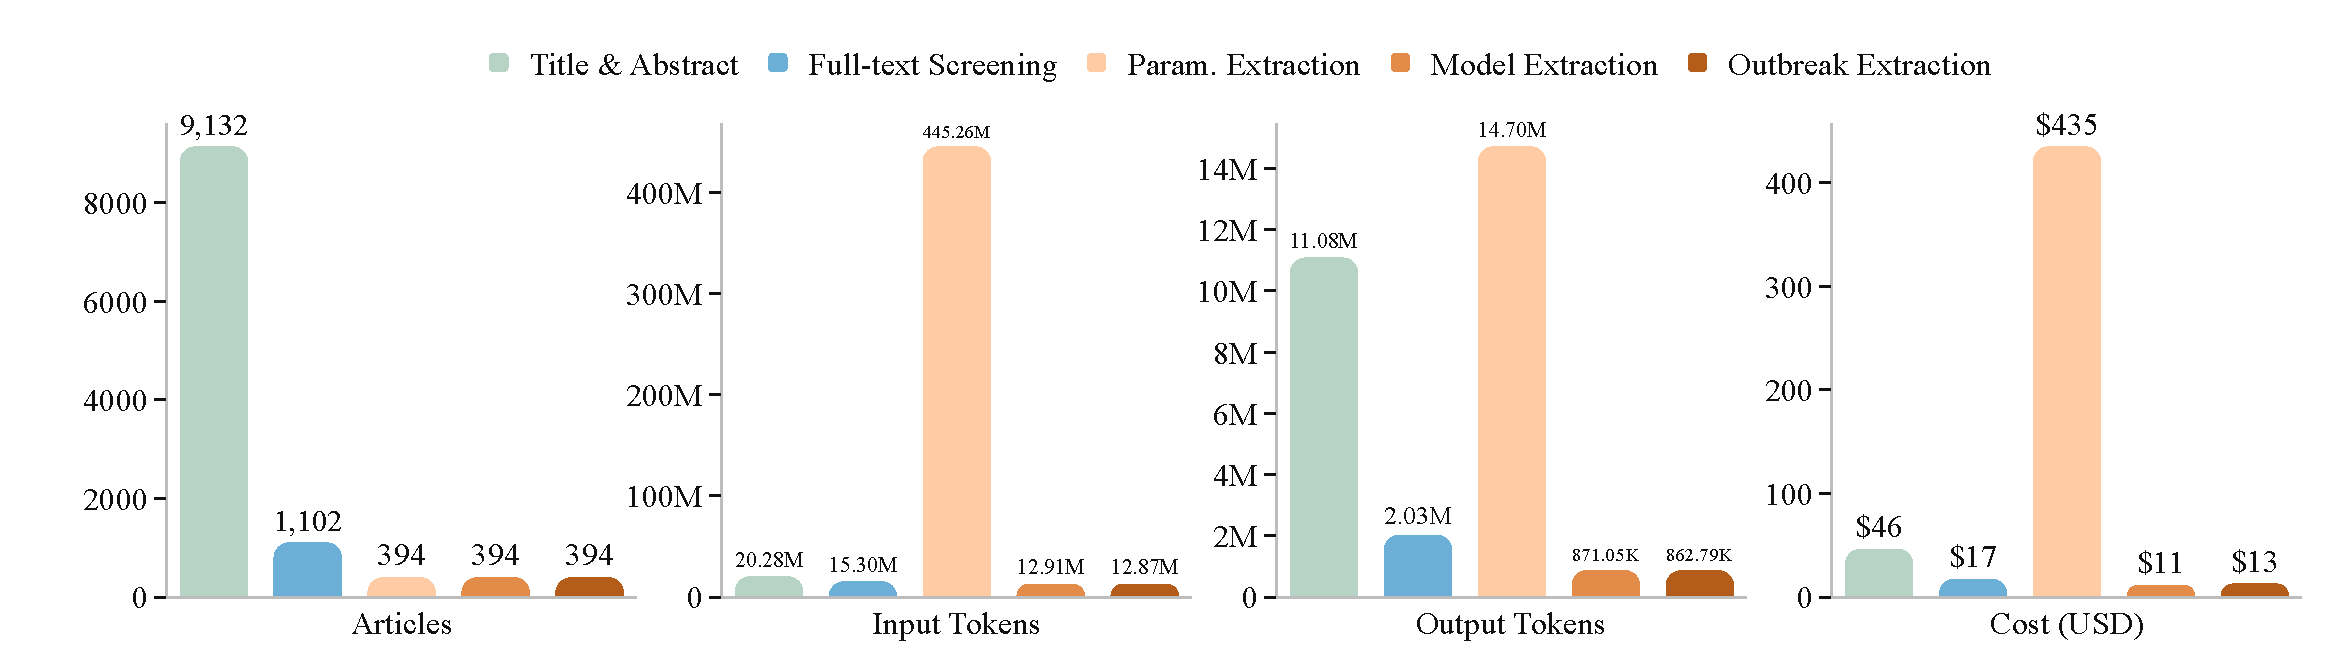
\includegraphics[width=\linewidth]{figures/pipeline_stats/token_articles_cost_by_stage.pdf}
    \caption{
\textbf{Articles processed, scaled token and costs by pipeline stage across models.}
We report the average number of articles reaching each stage, and the corresponding total input tokens, output tokens, and USD cost per stage averaged across models. Token totals are computed by multiplying per article token usage (Table~\ref{tab:token_usage_by_stage}) by the average article counts per stage (Table~\ref{tab:perg_slr_article_counts}).
Parameter extraction dominates overall compute, with substantially higher input and output token totals than other stages.
Title and abstract screening processes the largest volume of articles but contributes comparatively less to total cost.
}
    \label{fig:tokens_costs_articles_split}
\end{figure*}


Using the average article counts reported in Table~\ref{tab:perg_slr_article_counts}, we estimate total token usage and USD cost
across pipeline stages by combining per-article token statistics with model-specific
pricing. Figure~\ref{fig:tokens_costs_articles_split} summarises the resulting
distribution of articles processed, aggregate input tokens, output tokens, and total
cost by stage, averaged across models. Per-article input and output token usage by
stage and model is reported in Table~\ref{tab:token_usage_by_stage}. Total stage costs
are computed by multiplying mean per-article token usage by the average number of
articles reaching each stage, and then applying published per-million-token pricing
for both input and output tokens. All prices used in these calculations are retrieved
directly from the primary API pricing documentation of each model provider at the time
of evaluation.
Under this pricing regime, parameter extraction dominates overall compute and cost due
to substantially higher input and output token volumes, while title and abstract
screening processes the largest number of articles but contributes comparatively
little to total cost. All reported costs reflect managed API usage; alternative cost
estimates could be derived for deployments hosted on dedicated GPU nodes, where pricing
would depend on hardware configuration, utilisation, and amortisation assumptions
rather than per-token billing.

\footnotetext{
\textbf{GPT-OSS-120B:} \url{https://openrouter.ai/openai/gpt-oss-120b}. \\
\textbf{GPT-5.2:} \url{https://developers.openai.com/api/docs/pricing/}. \\
\textbf{DeepSeek-V3.2:} \url{https://api-docs.deepseek.com/quick_start/pricing}. \\
\textbf{Kimi-K2.5:} \url{https://platform.moonshot.ai/docs/pricing/chat}. \\
\textbf{GLM-4.7:} \url{https://docs.z.ai/guides/overview/pricing}.
}

% \SP{A) Mention in main-text the estimated costs are based on OpenRouter B) [Optional] Compute costs if self-hosted open-source models}



\begin{table*}[h]
\centering
\caption{
\textbf{Per article token usage and estimated cost by stage and model.}
We report mean input tokens, output tokens, and USD cost for processing a \textbf{single article} at each stage.
\highP{Green} marks the minimum and \lowP{Red} marks the maximum within each row and subcolumn.
}
\label{tab:token_usage_by_stage}
\setlength{\tabcolsep}{1.3pt}
\renewcommand{\arraystretch}{1.2}
{\footnotesize
\begin{tabular}{l|ccc|ccc|ccc|ccc|ccc}
\toprule
\textbf{Stage} & \multicolumn{3}{c|}{\textbf{GPT-OSS-120B (High)}} & \multicolumn{3}{c|}{\textbf{GPT-5.2 (High)}} & \multicolumn{3}{c|}{\textbf{DeepSeek-V3.2}} & \multicolumn{3}{c|}{\textbf{Kimi-K2.5}} & \multicolumn{3}{c}{\textbf{GLM-4.7}} \\
 & \makecell[c]{Input\\Tok.} & \makecell[c]{Output\\Tok.} & \makecell[c]{Cost\\(USD)} & \makecell[c]{Input\\Tok.} & \makecell[c]{Output\\Tok.} & \makecell[c]{Cost\\(USD)} & \makecell[c]{Input\\Tok.} & \makecell[c]{Output\\Tok.} & \makecell[c]{Cost\\(USD)} & \makecell[c]{Input\\Tok.} & \makecell[c]{Output\\Tok.} & \makecell[c]{Cost\\(USD)} & \makecell[c]{Input\\Tok.} & \makecell[c]{Output\\Tok.} & \makecell[c]{Cost\\(USD)} \\
\midrule
\makecell[l]{Title \& Abstract\\Screening} & \lowP{2.3K} & 1.2K& \highP{$<0.01$} & 2.2K& \highP{0.6K} & \lowP{0.01} & \highP{2.2K} & 0.6K& $<0.01$ & 2.3K& \lowP{2.0K} & $<0.01$ & 2.2K& 1.6K& $<0.01$ \\
\midrule
\makecell[l]{Article Screening\\(AI Conditioned)} & \lowP{16.9K} & 1.1K& \highP{$<0.01$} & 13.1K& 1.4K& \lowP{0.04} & \highP{12.9K} & \highP{0.8K} & $<0.01$ & 13.1K& 2.7K& 0.01 & 13.4K& \lowP{3.1K} & 0.01 \\
\midrule
\makecell[l]{Parameter\\Extraction} & \highP{510.2K} & 19.8K& \highP{0.02} & 961.1K& \lowP{91.1K} & \lowP{2.95} & 523.2K& \highP{3.0K} & 0.14 & 605.5K& 40.0K& 0.48 & \lowP{3050.4K} & 32.7K& 1.90 \\
\midrule
\makecell[l]{Model\\Extraction} & 35.9K& 1.9K& \highP{$<0.01$} & 31.5K& 2.1K& \lowP{0.08} & \lowP{37.2K} & \lowP{3.1K} & 0.01 & \highP{29.3K} & 2.2K& 0.02 & 29.7K& \highP{1.7K} & 0.02 \\
\midrule
\makecell[l]{Outbreak\\Extraction} & \lowP{49.9K} & 2.6K& \highP{$<0.01$} & 32.4K& \lowP{3.5K} & \lowP{0.10} & 26.1K& \highP{0.2K} & $<0.01$ & 29.5K& 2.7K& 0.02 & \highP{25.4K} & 2.0K& 0.01 \\
\midrule
\textbf{Overall} & 615.3K& 26.7K& \highP{0.02} & 1040.4K& \lowP{98.7K} & \lowP{3.20} & \highP{601.6K} & \highP{7.8K} & 0.17 & 679.8K& 49.6K& 0.55 & \lowP{3121.1K} & 41.1K& 1.96 \\
\bottomrule
\end{tabular}
}
\end{table*}
% \begin{itemize}
%     \item https://openrouter.ai/openai/gpt-oss-120b
%     \item https://platform.moonshot.ai/docs/pricing
%     \item https://developers.openai.com/api/docs/pricing/
%     \item https://docs.z.ai/guides/overview/pricing
%     \tem https://api-docs.deepseek.com/quick_start/pricing
% \end{itemize}

% PRICE_IN  = {'GPT-OSS-120B (High)':0.039,'GPT-5.2 (High)':1.75,'DeepSeek-V3.2':0.28,'Kimi-K2.5':0.6,'GLM-4.7':0.6}
% PRICE_OUT = {'GPT-OSS-120B (High)':0.19,'GPT-5.2 (High)':14.0,'DeepSeek-V3.2':0.42,'Kimi-K2.5':3.0,'GLM-4.7':2.2}





\clearpage

